\documentclass[12pt, titlepage]{article}

\usepackage{booktabs}
\usepackage{tabularx}
\usepackage{hyperref}
\usepackage{fancyhdr}
\pagestyle{fancy}

\hypersetup{
    colorlinks,
    citecolor=black,
    filecolor=blue,
    linkcolor=red,
    urlcolor=blue
}
\usepackage[round]{natbib}
\usepackage{graphicx}

\title{SE 3XA3: SRS\\Ultimate Tic Tac Toe}

\author{Team 3
		\\ Kunal Shah - shahk24
		\\ Pareek Ravi - ravip2
}

\date{\today}

%% Comments

\usepackage{color}

\newif\ifcomments\commentstrue

\ifcomments
\newcommand{\authornote}[3]{\textcolor{#1}{[#3 ---#2]}}
\newcommand{\todo}[1]{\textcolor{red}{[TODO: #1]}}
\else
\newcommand{\authornote}[3]{}
\newcommand{\todo}[1]{}
\fi

\newcommand{\wss}[1]{\authornote{blue}{SS}{#1}}
\newcommand{\ds}[1]{\authornote{red}{DS}{#1}}
\newcommand{\mj}[1]{\authornote{red}{MSN}{#1}}
\newcommand{\mh}[1]{\authornote{red}{MH}{#1}}
\newcommand{\cm}[1]{\authornote{red}{CM}{#1}}


% team members should be added for each team, like the following
% all comments left by the TAs or the instructor should be addressed
% by a corresponding comment from the Team

\newcommand{\tm}[1]{\authornote{magenta}{Team}{#1}}


\begin{document}
\lhead{Team 3 - System Requirement Specification}
\rhead{Ultimate Tic Tac Toe}
\maketitle

\pagenumbering{roman}
\tableofcontents
\listoftables
\listoffigures

\begin{table}[bp]
\caption{\bf Revision History}
\begin{tabularx}{\textwidth}{p{3cm}p{2cm}X}
\toprule {\bf Date} & {\bf Version} & {\bf Notes}\\
\midrule
October 3 & 1.0 & initial setup\\
October 5 & 1.1 & updated Project Drivers content\\
October 6 & 1.2 & added Functional Requirements\\
October 6 & 1.3 & added Non-functional Requirements\\
October 7 & 1.4 & updated Functional \& Non-functional Requirements\\
October 7 & 1.5 & Made notes for Project Issues\\
October 11 & 1.5 & finished for Project Issues\\
October 11 & 2.0 & Format document\\
\bottomrule
\end{tabularx}
\end{table}

\newpage

\pagenumbering{arabic}

\section*{Abstract}
This document describes the requirements for Ultimate Tic Tac Toe. The template 
for the Software Requirements Specification (SRS) is a subset of the Volere
template~\citep{RobertsonAndRobertson2012}.

\section{Project Drivers}

\subsection{The Purpose of the Project}
The purpose of this project is to redevelop an existing open source project
while following proper documentation and waterfall design methods.

\subsection{The Stakeholders}

The stakeholders include all parties that would have a vested interest in this
projected. This includes, the client Dr Smith, the developers Pareek and
Kunal ,all the people who would be interested in playing the game and the
teaching assistant Christopher.


\subsubsection{The Client}
The client of Ultimate Tic Tac Toe is Dr. Smith as he is the project manager and 
he requested this project. We are creating this game for him to distribute to 
the customer.

\subsubsection{The Customers}
The target customer for this game would be anyone who has a device connected to
the internet and wants to play a game with a friend. This game is targeted
towards young people, but it is open for anyone to play.

\subsubsection{Other Stakeholders}
Another stakeholder is the teaching assistant, Christopher, as is aiding Dr.
Smith in project management during lab and developers during the development 
process.

\subsection{Mandated Constraints}
There are 3 constraints of this game.	
\begin{enumerate}
	\item The internet
  	\item A device that can connect to the internet
  	\item A friend to play the game with
\end{enumerate}

\subsection{Naming Conventions and Terminology}
The naming convention for winning an inner game will be called controlling a
square. In order to win, a player must get a tic tac toe of controlled squares.
If there is a draw in a square, it will be called a dumped square.

\subsection{Relevant Facts and Assumptions}
We assume that the users have a stable internet connection and are aware of the
rules of regular Tic Tac Toe. It is important to note that the game will work
better in large screens rather than a small display. We assume that the user is
using a device that is either touch enables or has a mouse to click with.

\section{Functional Requirements}

\subsection{The Scope of the Work and the Product}

We investigated the original Ultimate tic tac toe game ~\citep{githubREF}. In
this  game the developer has poor user interface and no game instructions. It
also only supports single device with no AI option. These shortcomings are
the features we would like to improve upon.

\subsubsection{The Context of the Work}
The central task is to create a game of Ultimate Tic Tac Toe that can be played
on the internet with a friend. This will require a server to host the game, each
user to connect to the game, and ensure a connection with the server. In order
for the game to be played, the server will determine which player is to play,
get that player's move record it in the virtual board, and then notify the 
other player of the first player's move. This process of sending the move made 
back and forth will be the role of the server. The server will also indicate to
a player if they have won, lost or if that game has ended in a draw.

\subsubsection{Work Partitioning}
The development of this game is shared evenly between the two team members. The
game logic is developed by both members. The graphical portion is mainly going
to be done by Kunal, and the server portion will be done by Pareek.

\subsubsection{Individual Product Use Cases}
One of a possible use case is when a player might disconnect from their
internet connection, but their internet resumes and they wish to reconnect to
the game. Another case is if a player wished to change the device they are
playing on during an on going game. There could be a case where both players
agree that a player should be able to revert back by one move they made, in
which case the game will undo the user's last move. The general use case is of
course two users playing on their devices without any flaws from start to end.

\subsection{Functional Requirements}
Some of the functional requirements are that the game will display a game board
on the user's device, the user's move will be registered, recorded and
reflected on the game board. In addition, the game will determine when a player
has taken control of a square, when the square square is dumped and when the
game is won. The game logic will also determine in which square the next player
will make their move based on the previous player's move. In order for the game
to be played over the internet, the game would need to communicate to both
devices through means of a server.

\section{Non-functional Requirements}

\subsection{Look and Feel Requirements}
In order to make the game easy to use, clear instructions will be provided to
help them. With the use of unique but neutral colours, the aesthetics of the
game will also make it an enjoyable experience. Computers using a browser with
strong HTML5 support will be able to run the game easily. Interactive sounds
will be played when a user makes a move and to notify them that their opponent
has made their move. Smooth calming background music will also be played to make
the experience enjoyable.

\subsection{Usability and Humanity Requirements}
The game must have an easy UI which is not difficult to use or learn. Both the
touch interface and click interface should both work smoothly. There should a be
a tab for instructions on both the rules of the game and the game dynamic for 
those who do not know.

\subsection{Performance Requirements}
As this game will be played over the internet, it would be necessary for the
speed of the information transfer to be very fast. It would not be acceptable if
there was a long delay to record the move on another player's board. The game
board would also need to be constantly updated. If the game logic knows the
player's move, but it is not reflected on the board, that would be an issue.
When the user is using the touch interface, it is important to ensure that the
layout is such that the player does not accidentally make a move they did not
intend to make. A certain level of precision is required to ensure this doesn't
happen. Currently the game will be run on a local server, but in the future, a
larger server would be required to to match the demand for the game and ensure
that the server's capacity is sufficient. The server should be reliable and
available at all times such that it does not crash leaving people without the
ability to play the game.

\subsection{Operational and Environmental Requirements}
In order for the user to play this game, the system requirements are not very
high. As long as they are using a web browser (preferably Google Chrome) and
have a stable internet connection, the game should run smoothly. If the ping of
a user's internet is very poor, it would cause some issues in communicating with
the other player.

\subsection{Maintainability and Support Requirements}
The game should be easy to maintain as the only factor that would need constant
care is the server. The game logic is not complicated and would be simple to fix
if there were an error, but the server would be a challenge. If the server were
to reach capacity, it would take some time to transfer to a larger server. It is
currently impractical to use a large server for this product, but should the
demand rise, larger servers can be prepared to transfer over to.

\subsection{Security Requirements}
Since this game is being run over the internet, there is always the matter of
internet security. It is important that there be a certain level of encryption
to ensure that the information being transferred is safe and protected.

\subsection{Cultural Requirements}

The product shall not be offensive to religious or ethnic groups. The game user
interface should be language ambiguous. This means, even though the game is
provided in English, it should be able to be navigated and played by someone who
does not know how to read, write or speak English.

\subsection{Legal Requirements}
From a legal standpoint the main requirement is that we must not have access to
any personal information from the users from when they connect to the internet.
This game if it were to be rated by the ESRB, would have a rating of E for
everyone.

\subsection{Health and Safety Requirements}
When the game is being played, to ensure there is no possible cause of epilepsy
from the colors, very mild and neutral colors will be used to represent each
player. Majority of the health and safety is on the ownness of the user to
ensure they are not walking and playing or are not playing the game for
prolonged periods of time which could damage their health.

\section{Project Issues}

\subsection{Open Issues}
One issue we are concerned about is the adaptability of the user interface based
on the device. Some issues could arise from touch or mouse
input. Screen size of device could cause scaling problems such as having
part of the UI cut off. Lastly the user interface might not be the same based on
where the game is accessed. This could be caused due to the fact that different 
browsers render elements differently.

\subsection{Off-the-Shelf Solutions}
We will be utilizing four off the shelf solutions to assist this project 

\begin{enumerate}
	\item Moore server for web hosting
  	\item Gitlab for version control and issue tracking 
	\item Karma unit testing tool for verification 
	\item JsDoc for documentation generation
\end{enumerate}

\subsection{New Problems}
Some new problems that have arisen during the development process are user
problems such as miss click and poor internet connection. Additionally the
planned server is not powerful enough to cope with our projected growth pattern.

\subsection{Tasks}
The development cycle will follow the modified waterfall life cycle as detailed
by Dr. Smith. Refer to Figure \ref{fig:DevelopmentCycle}~\citep{Slides}. In
verification and validation, a set of test cases to ensure that all the game
features are working. Developing a thorough set of use cases as well as user
testing, the game will be tested. The design of this game will follow the
standard MVC game structure. The model will be located on the server, the view
and controller will be on each individual device. The code has been broken down
into various milestones. Please refer to the
\href{run:../../ProjectSchedule/Gantt Chart.gan}{Gantt Chart} for further
details. The final report will contain a detailed analysis of the result of the
test cases and the reviews from the test users.

\begin{figure}
  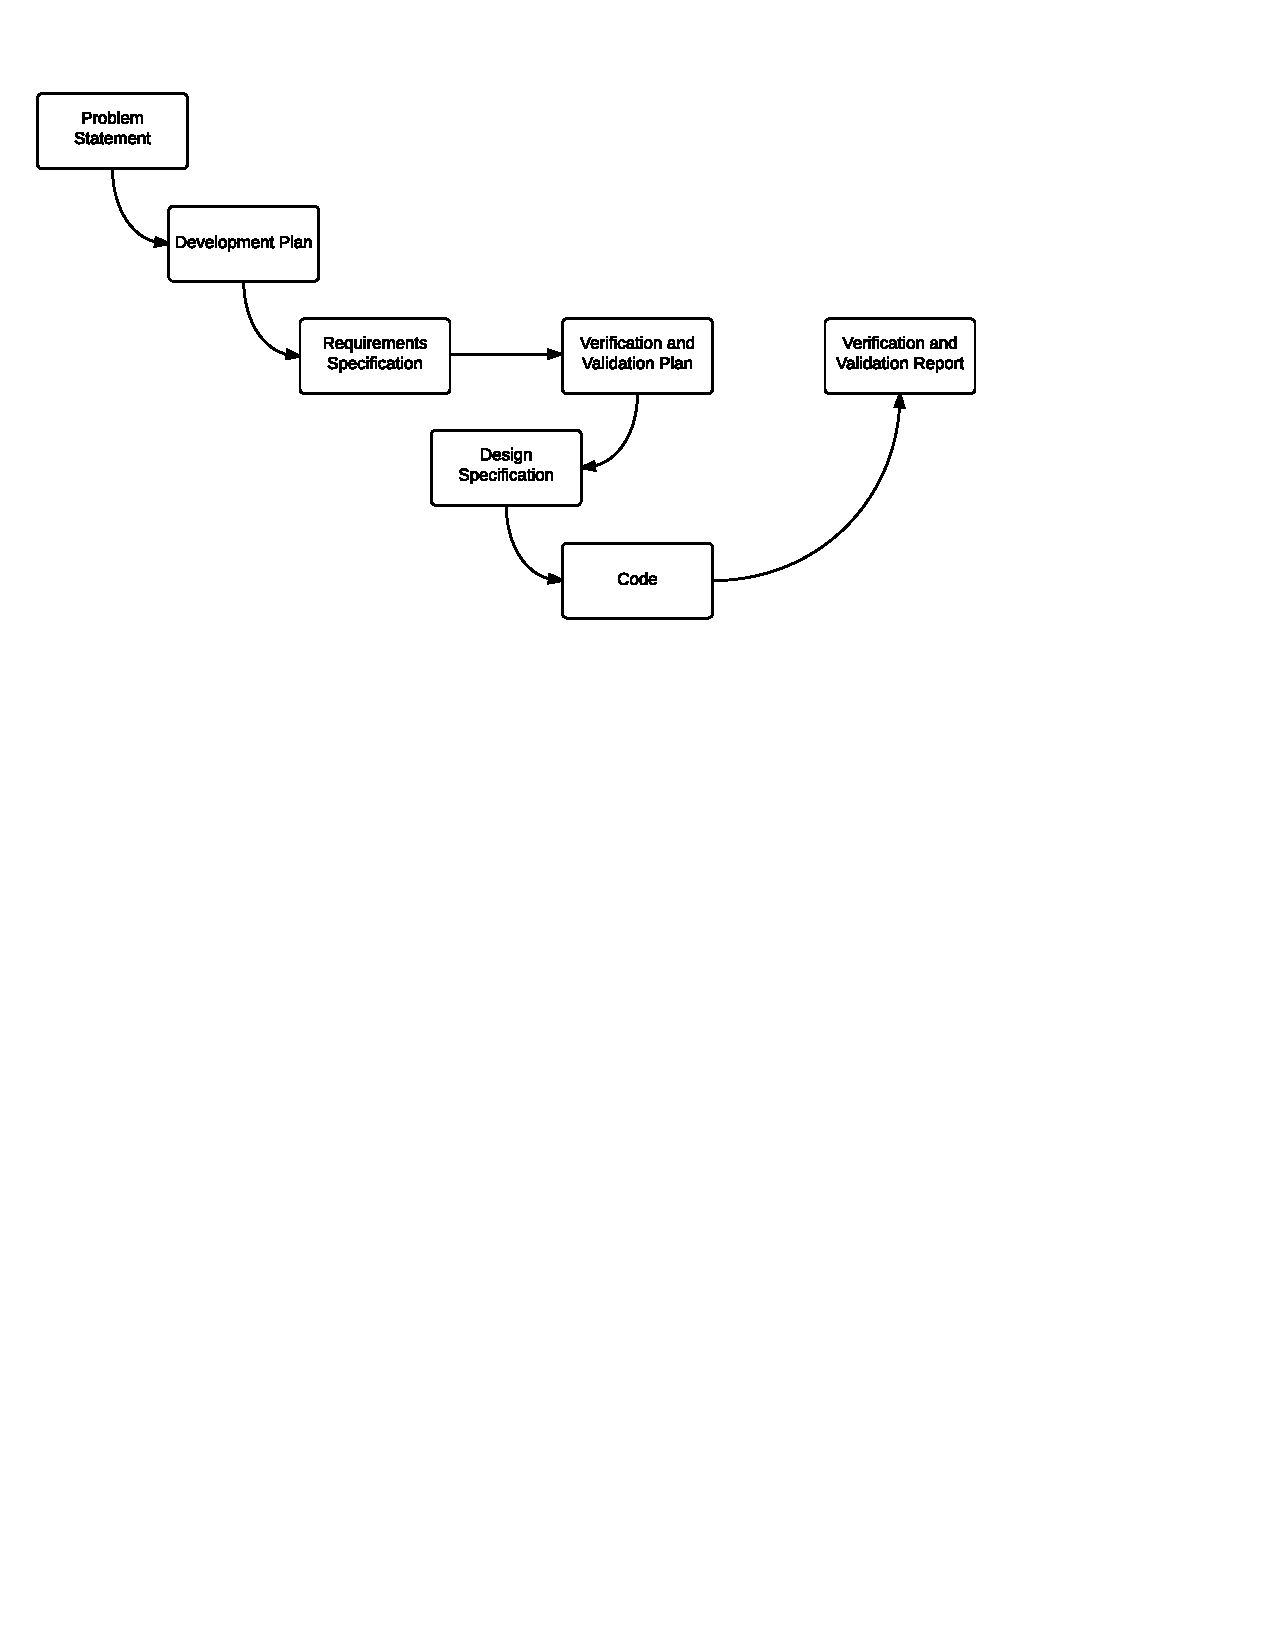
\includegraphics[width=\linewidth]{OverviewOfProcess.pdf}
  \caption{Development Cycle}
  \label{fig:DevelopmentCycle}
\end{figure}

\subsection{Migration to the New Product}
The migration to this project will involve transferring the game logic to the
server to allow for online game play if possible. The new product also will also
change the graphics and the user interface. From a MVC standpoint, the view is
the main change with the model shifting to the server. The controller will
remain the same except making it friendly for mobile devices and all touch
enabled devices.

\subsection{Risks}
There is a risk that the server that the game is hosted on could unexpectedly
crash. There is also a security risk with a device being connected insecurely to
the internet. We will ensure that only essential information is received and
there are minimal permissions

\subsection{Costs}
We plan to complete this project with a zero dollar budget. All resources used
to complete this project can be used free of charge. Additionally we plan to
host this game on the McMaster Moore server which is also available to us for
free.

\subsection{User Documentation and Training}
User documentation will be created in the form of game instructions.
Comprehensive game rules have already already been created by
mathwithbaddrawings.com~\citep{Rules} . Our game instructions will be a version
of theses rules with our own diagrams and explanations. There is no need for
user training.


\subsection{Waiting Room}
After redeveloping the Ultimate Tic Tac Toe game, we plan to add Player vs
Computer�� game mode. This AI should be able to intelligently perform moves based
on the human player's previous move. Secondly User accounts which will be able
to track player statistics such win ratio. Additionally we plan to add an online
lobby to face strangers. Players will be matched based on their player
statistics.

\subsection{Ideas for Solutions}
As discussed before we will be utilizing many off-the shelf solutions to help in
the development process. We plan to Use CSS to style the game board. To make the
game language ambiguous we will be including many images into the game
instructions. To make this game easy to maintain we shall be using
Model-��view-�controller (MVC) software architectural pattern to make it
modular.

\bibliographystyle{plainnat}

\bibliography{SRS}

\newpage

\section{Appendix}

\subsection{Symbolic Parameters}
MAX\_PLAYERS: Maximum number of concurrent players.


\end{document}